\hypertarget{premiers-pk-et-premiuxe8res-uxeeles-en-polynuxe9sie-franuxe7aise}{%
\section{Premiers Pk et premières îles en Polynésie
Française}\label{premiers-pk-et-premiuxe8res-uxeeles-en-polynuxe9sie-franuxe7aise}}

\emph{Vendredi 10 août 2018}

Cela fait maintenant une bonne semaine que nous sommes arrivés en
Polynésie Française. Je faisais partie des gens qui confondaient
\emph{Tahiti} avec \emph{Polynésie Française}. Après quelques jours ici,
j'ai bien pris conscience de la gaffe ! Réduire la Polynésie à une seule
île, ça ne marche tout simplement pas.

Nos premiers pas sur les îles se passent à Tahiti et Moorea.

\hypertarget{mapid}{}

Que dire de Tahiti alors ? Même si c'est le centre administratif de la
Polynésie Française, l'île elle-même est loin de l'image paradisiaque
associée à d'autres îles de l'archipel. Nous retiendrons quand même
quelques détails savoureux:

\begin{itemize}
\tightlist
\item
  il y a des chiens et des poules au bord de toutes les routes
\item
  tout le monde se lève avant 7 heures du matin (et se couche en
  conséquence)
\item
  quand on fait le tour de l'île, on trouve régulièrement des bornes
  appelées Pk, point kilométrique, qui permettent efficacement
  d'indiquer les localisations des points d'intérêt
\item
  on trouve des roulottes, sortes de food-truck immobilisés avec sièges
  et tables, un peu partout sur l'île et on y mange le plat national, le
  \emph{poisson cru coco}
\item
  les habitants de l'île sont tous très détendus, on est loin de
  l'esprit si commercial dont a l'habitude dans les lieux touristiques
  qu'on a fréquentés (même si évidemment le tourisme est ici aussi une
  manne)
\item
  on peut également faire de la randonnée sur l'île car le relief
  volcanique est très accidenté (nous en avons profité et sommes montés
  à la cascade de Loti)
\item
  il n'y a pas de plages partout, contrairement à ce que l'on pourrait
  penser, il faut un peu chercher pour les trouver (mais elles sont
  souvent magnifiques)
\end{itemize}

\begin{figure}
\centering
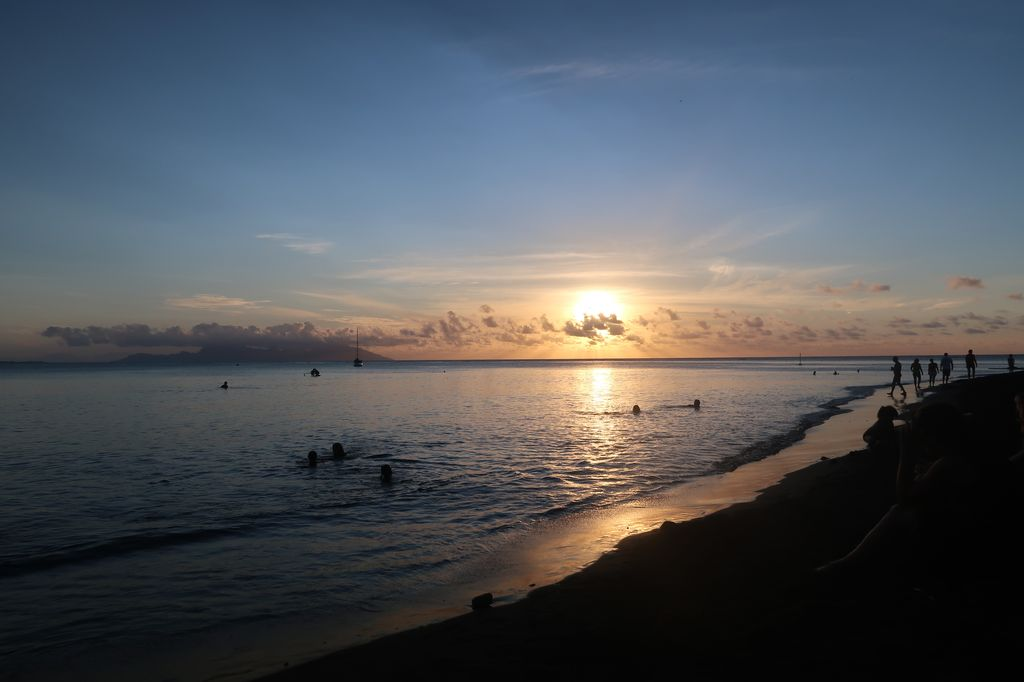
\includegraphics{images/20180810_tahiti.JPG}
\caption{En parlant de plages...}
\end{figure}

Nous retrouvons à Tahiti Guillaume et Camille avec qui nous voyagerons
pour les prochaines semaines.

Plus que Tahiti, c'est à Moorea que va notre coup de coeur de la
première semaine en Polynésie. A moins d'une heure en bateau de Tahiti,
et sur une surface bien plus petite, nous y avons passé quatre belles
journées. Cela est notamment dû à l'accueil parfait que nous a réservé
Laura, voyageuse espagnole en séjour longue durée à Moorea, dénichée via
AirBnb. Laura nous aura tout appris sur les attraits de l'île, y compris
comment préparer un poisson perroquet acheté en direct à son pêcheur
pour un barbecue réussi !

\begin{figure}
\centering
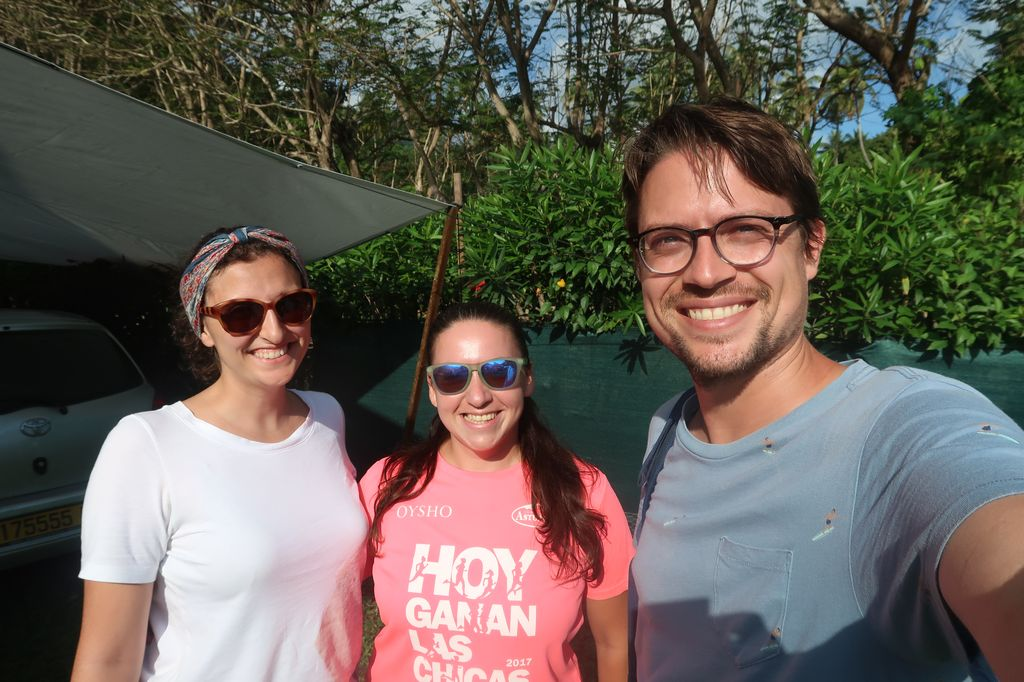
\includegraphics{images/20180810_moorea_laura.JPG}
\caption{Notre hôte à Moorea, Laura, le jour de notre départ.}
\end{figure}

Nous découvrons avec plaisir les différentes activités typiques des îles
polynésiennes : snorkeling avec les raies, mais aussi les requins (oui,
ça fait bizarre au début), tour de l'île tous les deux en scooter (mais
sans jamais dépasser quarante-cinq kilomètres à l'heure !), détente à la
plage de rêve de Temae, excursion pour faire du snorkeling et entendre
le chant des baleines. Ou encore visite de l'usine de jus de fruit
Rotui, qui fait la célébrité (et parfois la jalousie) de Moorea dans les
autres îles, observation astronomique depuis la terrasse quand le ciel
est clair et que s'ouvre au-dessus de nous la voie lactée. On découvre
aussi la météo qui peut être changeante : on passe facilement d'une
grosse averse qui fait mal (mais ne dure que dix minutes) au grand
soleil ! Et bien sûr les couchers de soleil sur la mer, dont on ne se
lasse pas...

Voilà donc les premières impressions d'ici. On enchaîne très bientôt
avec quatre jours à Bora-Bora, île du tourisme de luxe si l'on fait
confiance aux réputations !

\emph{Florian et Elida}
